\documentclass[8pt,a4paper,compress]{beamer}

\usepackage{/home/siyer/lib/slides}

\title{Merge Sort}
\date{}

\begin{document}
\begin{frame}
\vfill
\titlepage
\end{frame}

\begin{frame}
\frametitle{Outline}
\tableofcontents
\end{frame}

\section{Merging}
\begin{frame}[fragile]
\pause

Merge sort is based on a simple operation known as merging: combining two ordered arrays to make one larger ordered array

\pause
\bigskip

To sort an array, divide it into two halves, sort the two halves (recursively), and then merge the results

\pause
\bigskip

Merge sort overview
\begin{center}
\visible<4->{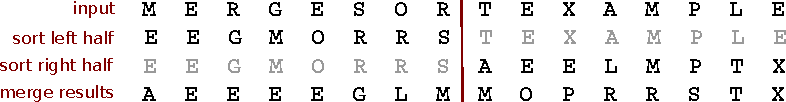
\includegraphics[scale=0.55]{{./figures/mergesort_overview}.pdf}}
\end{center}
\end{frame}

\begin{frame}[fragile]
\pause

The merge algorithm

\begin{lstlisting}[language=Java]
package edu.princeton.cs.algs4;

import java.util.Comparator;

public class Merge {
    private static void merge(Comparable[] a, Comparable[] aux, 
                              int lo, int mid, int hi) {
        int i = lo, j = mid + 1;
        for (int k = lo; k <= hi; k++) {
            aux[k] = a[k];
        }
        for (int k = lo; k <= hi; k++) {
            if (i > mid)                   { a[k] = aux[j++]; }
            else if (j > hi)               { a[k] = aux[i++]; }
            else if (less(aux[j], aux[i])) { a[k] = aux[j++]; }
            else                           { a[k] = aux[i++]; }
        }
    }
}
\end{lstlisting}
\end{frame}

\begin{frame}[fragile]
\pause

Trace of merge operation
\begin{center}

\visible<2->{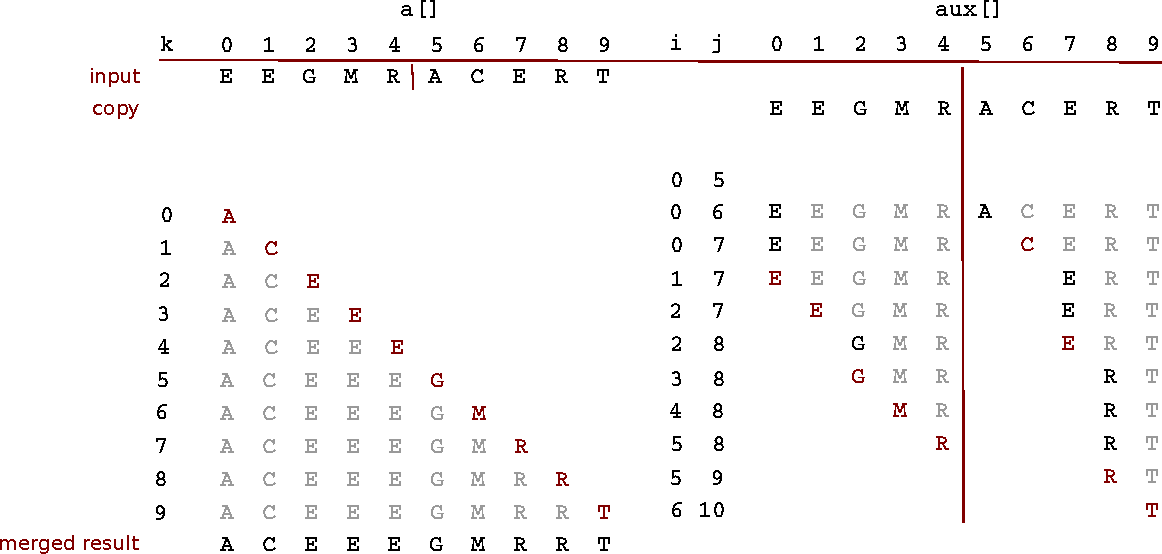
\includegraphics[scale=0.55]{{./figures/merge_trace}.pdf}}
\end{center}
\end{frame}

\section{Merge Sort}
\begin{frame}[fragile]
\pause

Top-down merge sort

\begin{lstlisting}[language=Java]
package edu.princeton.cs.algs4;

import java.util.Comparator;

public class Merge {
    public static void sort(Comparable[] a) {
        Comparable[] aux = new Comparable[a.length]; 
        sort(a, aux, 0, a.length - 1);
    }
    
    private static void sort(Comparable[] a, Comparable[] aux, 
                             int lo, int hi) {
        if (hi <= lo) { return; }
        int mid = lo + (hi - lo) / 2;
        sort(a, aux, lo, mid); 
        sort(a, aux, mid + 1, hi); 
        merge(a, aux, lo, mid, hi);
    }
}
\end{lstlisting}
\end{frame}

\begin{frame}[fragile]
\pause

Trace of merge sort
\begin{center}
\visible<2->{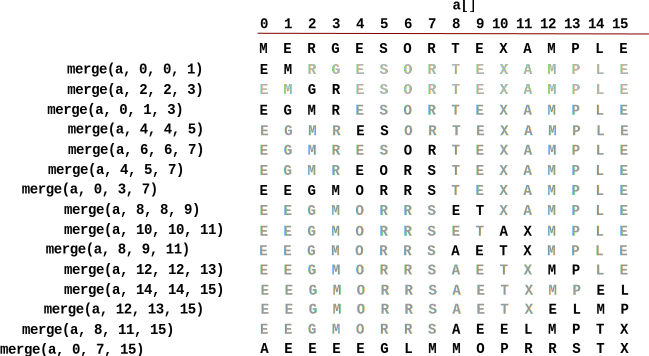
\includegraphics[scale=0.55]{{./figures/mergetd_trace}.pdf}}
\end{center}
\end{frame}

\begin{frame}[fragile]
\pause

Top-down merge sort uses $\sim N\lg N$ comparisons and $\sim N\lg N$ array accesses

\pause
\bigskip

The prime disadvantage of merge sort is that it uses extra space proportional to $N$

\pause
\bigskip

The \lstinline{MergeX} variant from the text implements the following improvements

\begin{itemize}
\item Handles tiny subarrays using insertion sort
\item Reduces the running time to be linear for arrays that are already in order by adding a test to skip the call to \lstinline$merge()$ if \lstinline$a[mid]$ is less than or equal to \lstinline$a[mid + 1]$
\item Eliminates the time taken to copy to the auxiliary array by switching the role of the input and auxiliary array in each recursive call
\end{itemize}
\end{frame}

\section{Complexity of Sorting}
\begin{frame}[fragile]
\pause

No comparison-based sorting algorithm can guarantee to sort $N$ items with fewer than $\lg N! \sim N\lg N$ comparisons

\pause
\bigskip

\begin{minipage}{150pt}
Proof: \begin{itemize}
\item Assume array consists of $N$ distinct values $a_1$ through $a_N$
\item Worst-case number of comparisons is dictated by height $h$ of decision tree
\item Binary tree of height $h$ has at most $2^h$ leaves
\item $N!$ different orderings $\implies$ at least $N!$ leaves
\item $N! \leq \text{number of leaves} \leq 2^h$
\item $\lg N! \leq h$, or using Stirling's approximation, $N\lg N \leq h$
\end{itemize}
\end{minipage}
\begin{minipage}{150pt}
\visible<3->{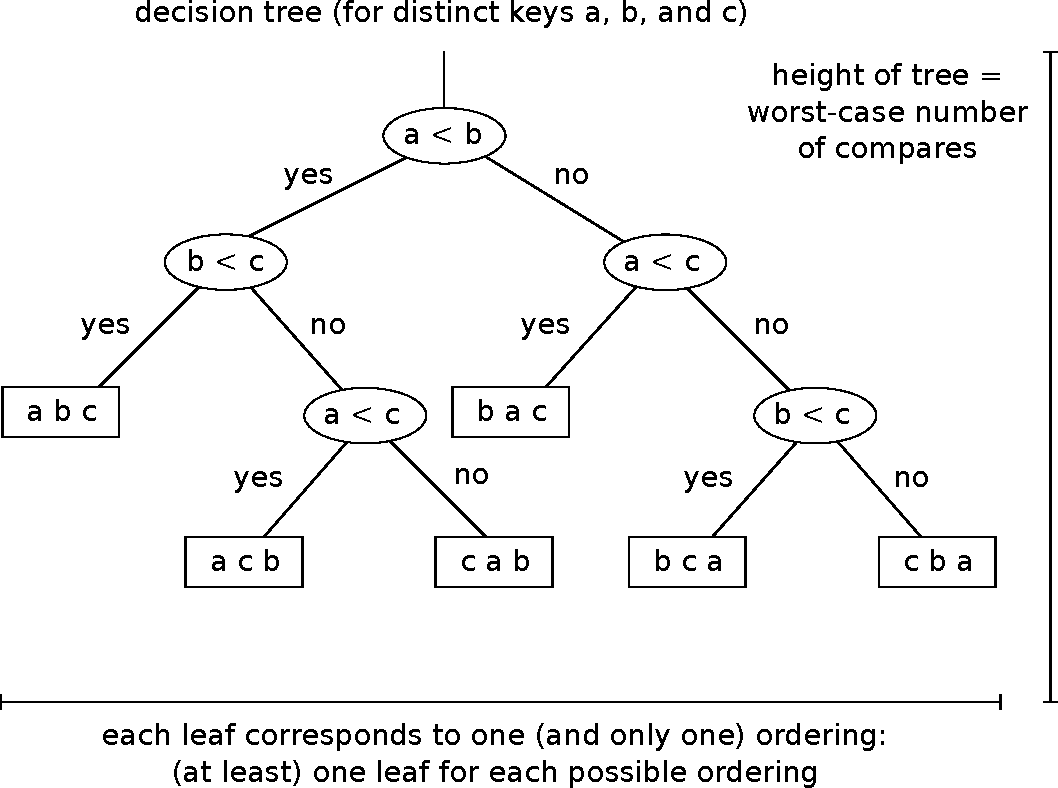
\includegraphics[scale=0.3]{figures/decision_tree.pdf}}
\end{minipage}

\pause
\bigskip

Merge sort is an asymptotically optimal comparison-based sorting algorithm, since the number of comparisons used by merge sort is $\sim N\lg N$
\end{frame}

\section{Merge Sort and Other Sorts}
\begin{frame}[fragile]
\pause

A comparison of merge sort and selection sort

\begin{lstlisting}[language={}]
$ java SortCompare Merge Selection 10000 100
For 10000 random Doubles
    Merge is 44.8 times faster than Selection
\end{lstlisting}

\pause
\bigskip

A comparison of merge sort and insertion sort
\begin{lstlisting}[language={}]
$ java SortCompare Merge Insertion 10000 100
For 10000 random Doubles
    Merge is 39.1 times faster than Insertion
\end{lstlisting}

\pause
\bigskip

A comparison of merge sort and shell sort

\begin{lstlisting}[language={}]
$ java SortCompare Merge Shell 10000 100
For 10000 random Doubles
    Merge is 1.1 times faster than Shell
\end{lstlisting}

\pause
\bigskip

A comparison of merge sort and system sort

\begin{lstlisting}[language={}]
$ java SortCompare Merge System 10000 100
For 10000 random Doubles
    Merge is 2.0 times faster than System
\end{lstlisting}
\end{frame}
\end{document}
